%%%%%%%%%%%%%%%%%%%%%%%%%%%%%%%%%%%%%%%%%%%%%%%%%%%%%%%%%%%%%%%%%%%%%%%%%%%%%%%%
%
%	Introduktion till TeX och LaTeX
%	Skriven av Viktor Ahlqvist
%	http://www.texempelvis.se
%
%	Baserat på en mall av Cameron Bracken.
%	Tänkt att användas med LuaTeX
%
%%%%%%%%%%%%%%%%%%%%%%%%%%%%%%%%%%%%%%%%%%%%%%%%%%%%%%%%%%%%%%%%%%%%%%%%%%%%%%%%

% Nag är ett paket som bör stå överst i alla dokument. Det tillför inga nya
% funktioner, men skriver varningar om man använder gamla, utdaterade,
% kommandon.
\RequirePackage[l2tabu, orthodox]{nag}

% För presentationer är klassen beamer väldigt användbar
\documentclass[xcolor=x11names,compress,swedish]{beamer}

%%%%%% Allmänna paket %%%%%%%%%%%%%%%%%%%%%%%%%%%%%%%%%%%%%%%%%%%%%%%%%%%%%%%%%%
% Grafik
\usepackage{graphicx}

% Matematik med amsmath
\usepackage{amsmath}

% Svenska översättningar med babel
\usepackage[swedish]{babel}

% Ladda typsnitt
\usepackage{fontspec}
\defaultfontfeatures{Mapping=tex-text, Ligatures={TeX,Common}}
\setmainfont[Numbers = OldStyle]{Open Sans}
\setsansfont{Fjalla One}
\setmonofont[Scale=MatchLowercase]{Inconsolata}
\newfontfamily\libertine[Numbers=OldStyle]{Linux Libertine O}

% Fixa matten med unicode-math
\usepackage[math-style=ISO,bold-style=ISO,vargreek-shape=unicode]{unicode-math}
\setmathfont{Asana Math}

% Fixa "problemet" med kommatecken som decimalavskiljare
\usepackage{icomma}

% siunitx är alltid trevligt att ha
%\usepackage{siunitx}

%csquotes
\usepackage[strict=true,style=swedish,swedish=quotes]{csquotes}

\usepackage{booktabs}

% Ritmöjligheter med TikZ
\usepackage{tikz}
\usetikzlibrary{decorations.fractals}

% Färger
\definecolor{dkgreen}{rgb}{0,0.6,0}
\definecolor{gray}{rgb}{0.5,0.5,0.5}
\definecolor{mauve}{rgb}{0.58,0,0.82}

% Listings, för kodexempel
\usepackage{listings}
\lstset{
	{language=[LaTeX]TeX},
	keywordstyle=\color{blue},
	commentstyle=\color{dkgreen},
	stringstyle=\color{mauve}
}

\newcommand*{\Lcode}{\lstinline[{language=[LaTeX]TeX}]}
\newcommand*{\Bashcode}{\lstinline[{language=Bash}]}
%%%%%%%%%%%%%%%%%%%%%%%%%%%%%%%%%%%%%%%%%%%%%%%%%%%%%%%%%%%%%%%%%%%%%%%%%%%%%%%%

%%%%%% Beamer-kommandon relaterade till utseendet %%%%%%%%%%%%%%%%%%%%%%%%%%%%%%
\useoutertheme[subsection=false,shadow]{miniframes}
\useinnertheme{default}
\usefonttheme{serif}

\setbeamerfont{title like}{shape=\scshape}
\setbeamerfont{frametitle}{shape=\scshape}

\setbeamercolor*{lower separation line head}{bg=DeepSkyBlue4} 
\setbeamercolor*{normal text}{fg=black,bg=white} 
\setbeamercolor*{alerted text}{fg=red} 
\setbeamercolor*{example text}{fg=black} 
\setbeamercolor*{structure}{fg=black} 
 
\setbeamercolor*{palette tertiary}{fg=black,bg=black!10} 
\setbeamercolor*{palette quaternary}{fg=black,bg=black!10} 


\setbeamertemplate{section in toc}[numbered]

% \renewcommand{\(}{\begin{columns}}
% \renewcommand{\)}{\end{columns}}
% \newcommand{\<}[1]{\begin{column}{#1}}
% \renewcommand{\>}{\end{column}}
%%%%%%%%%%%%%%%%%%%%%%%%%%%%%%%%%%%%%%%%%%%%%%%%%%%%%%%%%%%%%%%%%%%%%%%%%%%%%%%%

%%%%%% Lite egna kommandon om omdeklarationer %%%%%%%%%%%%%%%%%%%%%%%%%%%%%%%%%%
% Multiplication can be written either by a dot or a cross. Since the dot is
% the most common in Sweden, and since both are ok according to ISO, the dot
% is chosen (but that could of course be changed easily).
\AtBeginDocument{\let\times\cdot}

% According to the ISO standards, the 'd' in 'dx' in integrals should be written
% in upright, not italic or slanted. The following line adds the command \diff
% that typsets such a 'd'.
\newcommand*\diff{\mathop{}\!\mathrm{d}}

% Vectors could be written in several ways. TeX standard is to write them with
% a small arrow overhead. I prefer the bold letters, and I think ISO does that
% as well (but I can't confirm it at the moment).
\renewcommand{\vec}[1]{\ensuremath{\mathbf{#1}}}

%
\newcommand{\acr}[1]{{\small\MakeUppercase{#1}}}
%%%%%%%%%%%%%%%%%%%%%%%%%%%%%%%%%%%%%%%%%%%%%%%%%%%%%%%%%%%%%%%%%%%%%%%%%%%%%%%%

%%%%%% Metadata om dokumentet %%%%%%%%%%%%%%%%%%%%%%%%%%%%%%%%%%%%%%%%%%%%%%%%%%
\title{Typsättning med TeX och LaTeX}
%\subtitle{SUBTITLE}
\author{Viktor Ahlqvist\\\url{www.texempelvis.se}}
\date{12 april 2013}
%%%%%%%%%%%%%%%%%%%%%%%%%%%%%%%%%%%%%%%%%%%%%%%%%%%%%%%%%%%%%%%%%%%%%%%%%%%%%%%%

%%%%%% Hyperref och andra paket som laddas sist %%%%%%%%%%%%%%%%%%%%%%%%%%%%%%%%
\usepackage{hyperref}

\hypersetup{
	unicode,				% We want all strings in Unicode
	breaklinks,				% Allows line breaks in links
	pdfauthor = {Viktor Ahlqvist, www.texempelvis.se},	% Author of the document
	pdftitle = {Typsättning med TeX och LaTeX},	% Title of the document
	pdfsubject = {Typsättning med TeX och LaTeX},	% Subject
}
%%%%%%%%%%%%%%%%%%%%%%%%%%%%%%%%%%%%%%%%%%%%%%%%%%%%%%%%%%%%%%%%%%%%%%%%%%%%%%%%



%%%%%% Det egentliga innehållet %%%%%%%%%%%%%%%%%%%%%%%%%%%%%%%%%%%%%%%%%%%%%%%%
\begin{document}


\section{\scshape Introduktion}
\begin{frame}
	\titlepage
\end{frame}

%%%%%%%%%%%%%%%%%%%%%%%%%%%%%%%%%%%%%%%%%%%%%%%%%%%%%%%%%%%%%%%%%%%%%%%%%%%%%%%%
\begin{frame}{Disposition, mål och syfte}
	\begin{columns}[t]
		\begin{column}{0.5\textwidth}
			Disposition\\[2em]
			\setcounter{tocdepth}{1}
			{\small
				\tableofcontents
			}
		\end{column}
		% \hspace{0.1\textwidth}
		\begin{column}{0.5\textwidth}
			Syfte
			\begin{itemize}
				\item Kunna skriva enklare dokument
				\item Kunna skriva delar i större dokument
				\item Veta hur man söker mer information
			\end{itemize}
		\end{column}
	\end{columns}
\end{frame}

%%%%%%%%%%%%%%%%%%%%%%%%%%%%%%%%%%%%%%%%%%%%%%%%%%%%%%%%%%%%%%%%%%%%%%%%%%%%%%%%

\section{\scshape Om TeX}
\subsection{Bakgrund och terminologi}
	\begin{frame}[fragile]{En kort bakgrund}
		\begin{itemize}
			\item TeX skrivet av Donald Knuth under 1970-- och 1980-talet.
			\item Namnet kommer från grekiskans τεχνη
			\item Bygger på primitiva kommandon som kombineras i makron
			\item Exempel: \verb|\TeX|, som skriver ut \TeX{} blir
			\begin{lstlisting}
				T\kern -.1667em\lower .5ex\hbox{E}
				\kern -.125emX
			\end{lstlisting}
			\item LaTeX är en samling sådana makron
		\end{itemize}
	\end{frame}
	
	\begin{frame}{Terminologi}
		\begin{itemize}
			\item Motorn (engine)\\
					Det som typsätter dokumenten
			\begin{itemize}
				\item TeX
				\item e-TeX
				\item pdfTeX
				\item XeTeX
				\item LuaTeX
			\end{itemize}
			\item Format\\
					En samling makron som underlättar för användaren.
			\begin{itemize}
				\item plainTeX
				\item LaTeX
				\item ConTeXt
			\end{itemize}
			\item Distribution\\
					En samling av paket, motorer och externa program.
			\begin{itemize}
				\item TeX Live, alla operativsystem
				\item MiKTeX, Windows
				\item MacTeX, Mac OS
			\end{itemize}
		\end{itemize}
	\end{frame}
	
	\begin{frame}{Fördelar och nackdelar}
		Nackdelar
		\begin{itemize}
			\item Inte \acr{wysiwyg}
			\item Viss inlärningströskel
			\item Använda egna typsnitt var svårt
			\item Inte alltid lätt att få önskat utseende
		\end{itemize}
		\pause
		Fördelar
		\begin{itemize}
			\item Inte \acr{wysiwyg}
			\item Bra avstavningsalgoritm, snygga dokument
			\item Olika formatering från samma fil
			\item Automatiseringar!
			\item Fritt
		\end{itemize}
	\end{frame}
	
	\begin{frame}[fragile]{Arbetsflöde}
		\begin{enumerate}
			\item Skriv dokumentet i valfri textredigerare
			\item Typsätt dokumentet\\
					\Bashcode|$ lualatex dok|
			\item Kör eventuellt externa program\\
				\Bashcode|$ biber dok|\\
				\Bashcode|$ makeglossaries dok|
			\item Typsätt dokumentet igen\\
				\Bashcode|$ lualatex dok|
			\item Visa pdf-filen i t.ex. Adobe Acrobat
		\end{enumerate}
	\end{frame}

%%%%%%%%%%%%%%%%%%%%%%%%%%%%%%%%%%%%%%%%%%%%%%%%%%%%%%%%%%%%%%%%%%%%%%%%%%%%%%%%

\section{\scshape Grundläggande LaTeX}
	\subsection{Hello world}
		\begin{frame}[fragile]{Ett första exempel}
			\begin{columns}
				\begin{column}{0.5\textwidth}
						\lstinputlisting[
							basicstyle=\tiny,
							numbers=left,
							numberstyle=\tiny\color{gray},
							stepnumber=1,
							numbersep=5pt]{examples/example1.tex}
				\end{column}
				\begin{column}{0.5\textwidth}
					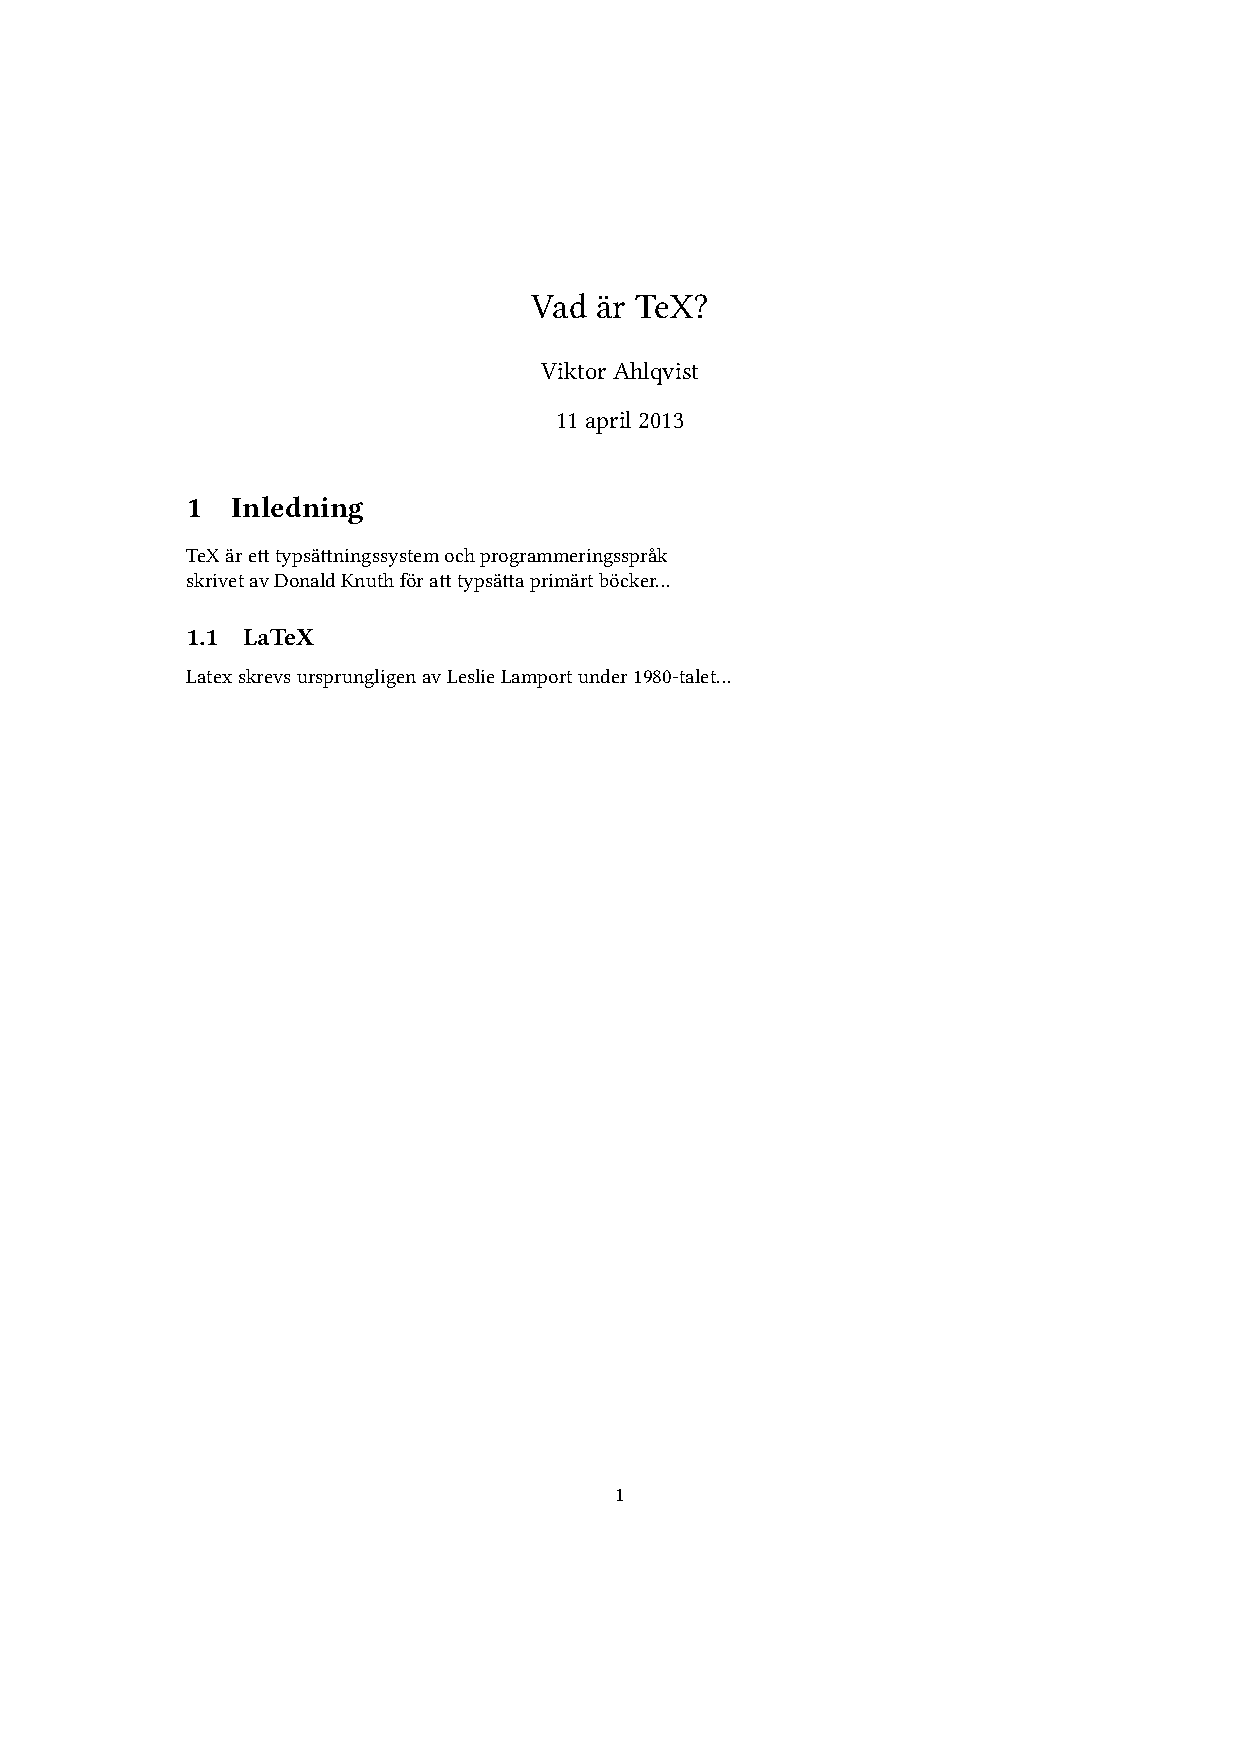
\includegraphics[trim=5cm 5cm 5cm 5cm, width=\textwidth]{examples/example1.pdf}
				\end{column}
			\end{columns}
		\end{frame}
			
		\begin{frame}[fragile]{Mellanrum, kommentarer och nyrader}
			\begin{columns}
				\begin{column}{0.5\textwidth}
						\lstinputlisting[
							basicstyle=\tiny,
							numbers=left,
							numberstyle=\tiny\color{gray},
							stepnumber=1,
							numbersep=5pt,
							showspaces=true,
							showtabs=true]{examples/example2.tex}
				\end{column}
				\begin{column}{0.5\textwidth}
					
\includegraphics[trim=5cm 8cm 5cm 2cm, width=\linewidth]{examples/example2.pdf}
				\end{column}
			\end{columns}
		\end{frame}
		
		\begin{frame}{Tio reserverade tecken}
			\begin{tabular}{lll}
				Tecken & Användning & Kommando\\ \toprule
				\#	& parameterreferens	& \textbackslash\#\\
				\$	& byter till matteläge	& \textbackslash\$\\
				\%	& kommentar	& \textbackslash\%\\
				\&	& justering (t.ex. i tabeller)	& \textbackslash\&\\
				\textasciitilde & hårt mellanrum	& \textbackslash textasciitilde\\
				\_	& index (matteläge)	& \textbackslash\_\\
				\textasciicircum & exponent (matteläge)	& \textbackslash textasciicircum\\
				\{	& gruppering, start	& \textbackslash\{\\
				\}	& gruppering, slut	& \textbackslash\}\\
				\textbackslash & start kommando	& \textbackslash textbackslash, \textbackslash backslash
			\end{tabular}
		\end{frame}
	
	% \subsection{Kommandon}
	% 	\begin{frame}[fragile]{Dokumentstruktur}
	% 		\begin{itemize}
	% 			\item Ingress \emph{(preamble)}
	% 			\begin{itemize}
	% 				\item Dokumentklass \Lcode|\documentclass[]{}|
	% 				\item Ladda paket \Lcode|\usepackage[]{}|
	% 				\item Inställningar
	% 			\end{itemize}
	% 			\item Huvuddelen
	% 			\begin{itemize}
	% 				\item Inledning \emph{(front matter)}
	% 				\begin{itemize}
	% 					\item titelsida
	% 					\item abstrakt
	% 				\end{itemize}
	% 				\item Huvuddel \emph{(main matter)}
	% 				\item Avslutning \emph{(back matter)}
	% 				\begin{itemize}
	% 					\item appendix
	% 					\item bibliografi
	% 				\end{itemize}
	% 			\end{itemize}
	% 		\end{itemize}
	% 	\end{frame}
		
		\begin{frame}[fragile]{Textstorlek}
			\begin{columns}[t]
				\begin{column}{0.5\textwidth}
					\begin{tabular}{ll}
						Storlek		& 	Exempel\\ \toprule
						tiny		&	{\tiny Exempel}\\
						scriptsize	&	{\scriptsize Exempel}\\
						footnotesize &	{\footnotesize Exempel}\\
						small		&	{\small Exempel}\\
						normalsize	&	{\normalsize Exempel}\\
						large		&	{\large Exempel}\\
						Large		&	{\Large Exempel}\\
						LARGE		&	{\LARGE Exempel}\\
						huge		&	{\huge Exempel}\\
						Huge		&	{\Huge Exempel}
					\end{tabular}
				\end{column}
				\begin{column}{0.4\textwidth}
					Kan användas antingen som en \emph{switch} eller som en \emph{environment}.
					{\small
					\begin{lstlisting}
						{\small En liten text}
						\begin{small}
							en annan liten text
						\end{small}
					\end{lstlisting}
					}
				\end{column}
			\end{columns}
		\end{frame}
		
		\begin{frame}[fragile]{Texttyper}
			\begin{tabular}{lll}
				Switch				& Kommando			& Exempel \\ \toprule
				\Lcode|\mdseries|	& \Lcode|\textmd|	& {\libertine\mdseries Mellanfet stil}\\
				\Lcode|\normalfont| & \Lcode|\textnormal| & {\libertine Normal stil}\\
				\Lcode|\rmfamily|	& \Lcode|\textrm|	& {\libertine Rak stilsort}\\
				\Lcode|\upshape|	& \Lcode|\textup|	& {\libertine\upshape Rak stil}\\
				\Lcode|\itshape|	& \Lcode|\textit|	& {\libertine\itshape Kursiv stil}\\
				\Lcode|\slshape|	& \Lcode|\textsl|	& {\libertine\slshape Snedställd stil}\\
				\Lcode|\bfseries|	& \Lcode|\textbf|	& {\libertine\bfseries Fet stil}\\
				\Lcode|\scshape|	& \Lcode|\textsc|	& {\libertine\scshape Kapitäler}\\
				\Lcode|\sffamily|	& \Lcode|\textsf|	& {\sffamily Sans-serif}\\
				\Lcode|\ttfamily|	& \Lcode|\texttt|	& {\ttfamily Skrivmaskinsstil}
			\end{tabular}
		\end{frame}
		
		\begin{frame}[fragile]{Texttyper}
			\begin{itemize}
					\item[] Antalet former och stilar begränsas av typsnittens.
					\begin{columns}
						\small
						\begin{column}{0.5\textwidth}
							\item[] Stilsort \emph{(font family)}
							\begin{itemize}
								\item \Lcode|\rmfamily|
								\item \Lcode|\sffamily|
								\item \Lcode|\ttfamily|
							\end{itemize}
							\item[] Vikt \emph{(series, weight)}
							\begin{itemize}
								\item \Lcode|\mdseries|
								\item \Lcode|\bfseries|
							\end{itemize}
							\item[]
							\item[] Exempel på \emph{switch}\\
								\Lcode|{\ttfamily exempeltext}|
						\end{column}
						\begin{column}{0.5\textwidth}
							\item[] Stil, form \emph{(shape)}
							\begin{itemize}
								\item \Lcode|\upshape|
								\item \Lcode|\itshape|
								\item \Lcode|\slshape|
								\item \Lcode|\scshape|
							\end{itemize}
							\item[] Normal stilsort, vikt och form
							\begin{itemize}
								\item \Lcode|\normalfont|
							\end{itemize}
							\item[]
							\item[] Exempel på kommando\\
								\Lcode|\texttt{exempeltext}|
						\end{column}
					\end{columns}
					\Lcode|\emph{...}| eller \Lcode|\textit{...}|
				\end{itemize}
		\end{frame}
		
		\begin{frame}[fragile]{Rubriker}
			\begin{tabular}{lll}
				Kommando				& Nivå\\ \toprule
				\Lcode|\part{}|			& -1\\
				\Lcode|\chapter{}|		& 0 & endast i bok \& rapport\\
				\Lcode|\section{}|		& 1\\
				\Lcode|\subsection{}|	& 2\\
				\Lcode|\subsubsection{}|& 3\\
				\Lcode|\paragraph{}|	& 4\\
				\Lcode|\subparagraph{}|	& 5\\
				~\\
				\Lcode|\section*{}|\\
				\Lcode|\section[kort text]{lång text}|
			\end{tabular}
		\end{frame}

		\begin{frame}[fragile]{Justering av text}
			\begin{itemize}
				\item Normalt är justering av båda marginaler
				\item Centrering
				\begin{itemize}
					\item \Lcode|\begin{center} Centrerad text \end{center}|
					\item \Lcode|\centering|
				\end{itemize}
				\item Vänsterjusterad
				\begin{itemize}
					\item \Lcode|\begin{flushleft} Vänsterjusterad text \end{flushleft}|
					\item \Lcode|\raggedright|
				\end{itemize} 
				\item Högerjusterad
				\begin{itemize}
					\item \Lcode|\begin{flustright} Högerjusterad text \end{flustright}|
					\item \Lcode|\raggedleft|
				\end{itemize}
			\end{itemize}
		\end{frame}
		
		\begin{frame}[fragile]{Tabeller}
			\begin{itemize}
				\item tabular
				\begin{lstlisting}
					\begin{tabular}[<global>]{<kolumnjustering>}
						text & text & text & text\\
						text & text & text & text\\
					\end{tabular}
				\end{lstlisting}
				\item global placering
				\begin{itemize}
					\item[] Vertikal global placering, \Lcode|t|, \Lcode|c| eller \Lcode|b|
				\end{itemize}
				\item kolumnjustering
				\begin{itemize}
					\item[] \Lcode|l| vänsterjusterad
					\item[] \Lcode|r| högerjusterad
					\item[] \Lcode|c| centrerad
					\item[] \Lcode|p{<bredd>}| En <bredd>-bred text
					\item[] \Lcode+|+ en vertikal linje. Bör en användas!
				\end{itemize}
				
				% \item tabular*
				% \item array
				% \item longtable
			\end{itemize}
		\end{frame}

		\begin{frame}[fragile]{Mer tabeller}
			Exempel
			\begin{lstlisting}
				\begin{tabular}{lp{2.5cm}r}
					Vara	& Beskrivning & Pris \\ \hline
					Magnum	& Glass, glass i stora lass!		  & 23 kr\\
					Hönökaka& Bröd		  & 16 kr\\
				\end{tabular}
			\end{lstlisting}
			
			\begin{tabular}{lp{2.5cm}r}
				Vara	& Beskrivning & Pris \\ \hline
				Magnum	& Glass, glass i stora lass!		  & 23 kr\\
				Hönökaka& Bröd		  & 16 kr\\
			\end{tabular}
		\end{frame}

		\begin{frame}[fragile]{Än mer tabeller}
			\begin{itemize}
				\item \Lcode|\multicolumn{antal}{<kolumnjustering>}{text}|
				\item \texttt{tabular*}, \texttt{tabularx}\\
					Låter en specificera bredden på tabellen.
				\item \texttt{longtable}\\
					Tabeller som kan sidbrytas och mycket mycket mer
				\item \texttt{booktabs}\\
					Bättre linjer
			\end{itemize}
		\end{frame}
		
		\begin{frame}[fragile]{Etiketter och referenser}
			\begin{itemize}
				\item Etiketter kan läggas i stort sett var som helst i dokument
				\item Latex bestämmer vad som ska refereras
				\item \Lcode|\label{sec:inledning}|\\
					  \Lcode|\ref{sec:inledning}|
				\item Vanligt att använda
				\begin{itemize}
					\item \texttt{sec:} för sektioner
					\item \texttt{fig:} för figurer
					\item \texttt{eq:} för ekvationer
				\end{itemize}
				\item Bättre referenser med \texttt{cleverref}
				\begin{itemize}
					\item \Lcode|\cref{sec:inledning}|
				\end{itemize}
			\end{itemize}
		\end{frame}	
	
		\begin{frame}[fragile]{Float}
			\begin{itemize}
				\item \texttt{table}, \texttt{figure}
				\item Position bestäms automatiskt
				\item Rangordna positioner, \texttt{h, t, b, p, !}
				\begin{lstlisting}
					\begin{figure}[htbp]
						\includegraphics{bild2}
					\end{figure}
				\end{lstlisting}
				\item \Lcode|\caption[...]{...}|
				\item \Lcode|\label{}|
			\end{itemize}
		\end{frame}

		\begin{frame}[fragile]{Punktlistor}
			\begin{itemize}
				\item \texttt{enumerate}, \texttt{itemize}
				\item \Lcode|\item ...|, \Lcode|\item[] ...|
				\begin{lstlisting}
					\begin{itemize}
						\item \texttt{enumerate}, \texttt{itemize}
						\item \Lcode|\item ...|, \Lcode|\item[] ...|
					\end{itemize}
				\end{lstlisting}
			\end{itemize}
		\end{frame}
		\begin{frame}[fragile]{Andra språk}
			\begin{itemize}
				\item \texttt{babel}
				\begin{itemize}
					\item \Lcode|\usepackage[swedish]{babel}|
					\item \Lcode|\usepackage[swedish,UKenglish]{babel}|
					\item byt språk med \Lcode|\selectlanguage{swedish}|
				\end{itemize}
				\item \texttt{polyglossia}, endast Xetex i nuläget
					\begin{itemize}
						\item \Lcode|\usepackage{polyglossia}|
						\item \Lcode|\setdefaultlanguage{swedish}|
					\end{itemize}				
			\end{itemize}
		\end{frame}
		
		\begin{frame}[fragile]{Bindestreck och citattecken}
			\begin{itemize}
				\item Typografiska ``citattecken'' med \verb|``citerad text''|
				\item Luatex, Xetex stöder UTF-8
				\item[]
				\item \Lcode|-| bindestreck/divis, -
				\item \Lcode|--| tankstreck, --
				\item \Lcode|---| långt tankstreck, ---
			\end{itemize}
		\end{frame}
		
		\begin{frame}[fragile]{Inkludera andra filer}
			\begin{itemize}
				\item \Lcode|\include{...}|
				\item \Lcode|\includeonly{...,...}|
				\item \Lcode|\input{...}|
				\item[]
				\item Speciella dokumentklasser
				\begin{itemize}
					\item \texttt{subfile}
					\item \texttt{standalone}
				\end{itemize}
			\end{itemize}
		\end{frame}
		
		\begin{frame}[fragile]{Nya kommandon}
			\begin{itemize}
				\item Egna kommandon kan och bör skapas
				\item \Lcode|\newcommand{\acr}[1]{\textsc{#1}}|
				\item \Lcode|\newcommand{\companyname}{Företaget AB}|
				\item \Lcode|\renewcommand{\companyname}{Annat företag AB}|
				\item \Lcode|\def| bör inte användas!
			\end{itemize}
		\end{frame}
%%%%%%%%%%%%%%%%%%%%%%%%%%%%%%%%%%%%%%%%%%%%%%%%%%%%%%%%%%%%%%%%%%%%%%%%%%%%%%%%
\section{\scshape Matematik}
	\subsection{Matematikläge}
		\begin{frame}[fragile]{Matematikläge}
			\begin{itemize}
				\item AMS-Latex\\
					\Lcode|\usepackage{amssmath}|, samling av 6 paket.
				\item Tre lägen i Latex
				\begin{itemize}
					\item Vanlig text
					\item Matte i text, \Lcode|$ ... $| eg. \Lcode|\( ... \)|
					\item Matte (display)
				\end{itemize}
				\item $\sum^n_{i=0} \binom{n}{i} a^i b^{n-i} = (a + b)^n$\\
				\begin{equation}
					\sum^n_{i=0} \binom{n}{i} a^i b^{n-i} = (a + b)^n
				\end{equation}
				\begin{lstlisting}[{language=[LaTeX]TeX},showspaces=true,showtabs=true]
					$\sum^n_{i=0}\binom{n}{i}       a^i
					b^{n-i} = (   a +  b)^n$
				\end{lstlisting}
			\end{itemize}
		\end{frame}
		
		\begin{frame}[fragile]{Index och potenser}
			\begin{itemize}
				\item Index fås med \Lcode|_|
				\item Flera tecken grupperas med \Lcode|{n+1}|
				\item Potenser fås med \Lcode|^|
				\item Kan kombineras
				\item \Lcode|\phantom{}| för mellanrum\\
					$x_0^2$ eller $x_0^{\phantom{2}2}$\\
					\Lcode|x_0^{\phantom{2}2}| 
			\end{itemize}
		\end{frame}
		
		\begin{frame}[fragile]{Grekiska bokstäver}
			\begin{itemize}
				\item Gemener: $\alpha$ (\Lcode|\alpha|), $\beta$ (\Lcode|\beta|), $\phi$ (\Lcode|\phi|)
				\item Alternativa: $\varepsilon$ (\Lcode|\varepsilon|), $\varphi$ (\Lcode|\varphi|)
				\item Versaler: $\Alpha$ (\Lcode|\Alpha|), $\Beta$ (\Lcode|\Delta|), $\Phi$ (\Lcode|\Phi|)
				\item \texttt{unicode-math} löser ``problem''
			\end{itemize}
		\end{frame}
		
		\begin{frame}{Olika mattelägen}
			\begin{itemize}
				\item \texttt{equation} enradesekvationer
				\item \texttt{equation*} utan numrering
				\item \texttt{align} flera rader och justeringar
				\item \texttt{gather} flera rader utan justering
				\item \texttt{eqnarray} bör \emph{inte} användas
			\end{itemize}
		\end{frame}
		
		\begin{frame}[fragile]{aligned}
			Byggblock i andra ekvationer
			\begin{equation*}
				I = \left[
				\begin{aligned}
					1 && 0 && 0 \\ 0 && 1 && 0 \\
					0 && 0 && 1
				\end{aligned}
				\right]
			\end{equation*}
			\begin{lstlisting}
				\begin{equation*}
					I = \left[
					\begin{aligned}1 && 0 && 0 \\
						0 && 1 && 0 \\0 && 0 && 1
					\end{aligned}
					\right]
				\end{equation*}
			\end{lstlisting}
		\end{frame}
		
		\begin{frame}[fragile]{left - right}
			\begin{itemize}
				\item Automatisk skalning av parenteser
				\item \Lcode|\left(|, \Lcode|\right)|
				\item \Lcode|\left(|, \Lcode|\right.|
				\begin{equation*}
					n! = \left\{
					\begin{aligned}
					& 1 && \text{if $0 \leq n \leq 1$},
					\\ & n \times (n-1)! && \text{otherwise}. \end{aligned}
					\right.
				\end{equation*}
			\end{itemize}
		\end{frame}

%%%%%%%%%%%%%%%%%%%%%%%%%%%%%%%%%%%%%%%%%%%%%%%%%%%%%%%%%%%%%%%%%%%%%%%%%%%%%%%%
% \section{\scshape Mer LaTeX}
% 	\subsection{Klasser och paket}
% 		\begin{frame}{Dokumentklasser}
% 		\end{frame}
% 
% 	\subsection{Arbetsflöden}
% 		\begin{frame}{Inkludera filer}
% 		\end{frame}
% 
% %%%%%%%%%%%%%%%%%%%%%%%%%%%%%%%%%%%%%%%%%%%%%%%%%%%%%%%%%%%%%%%%%%%%%%%%%%%%%%%%		
\section{\scshape Externa program}
	\subsection{Referenshantering}
		\begin{frame}{BibTeX - BibLaTeX}
			\begin{itemize}
				\item Referenshanteringssystem
				\item Externt program
				\begin{itemize}
					\item BibTeX
					\item Biber
				\end{itemize}
				\item Ladda färdiga stilar, t.ex. \texttt{ieee}
			\end{itemize}
		\end{frame}


\section{\scshape Avslutning}
	\subsection{Avslutning}
		\begin{frame}{Avslutning}
			\begin{itemize}
				\item Wikibooks Latex-bok\\
				\item Latex and friends av M.R.C van Dongen
				\item[]
				\item LaTeX-tips av Malin Palö och Niklas Andersson, GU-matte\\
				\item Att TeXa: en praktisk guide av Simon Sigurdhsson, fysik\\
				\item Att skriva rapporter med LaTeX av Per Foreby, Lunds universitet\\
				\item[]
				\item TeXempelvis, \url{http://www.texempelvis.se}
			\end{itemize}
		\end{frame}



\end{document}




%%%%%%%%%%%%%%%%%%%%%%%%%%%%%%%%%%%%%%%%%%%%%%%%%%%%%%%%%%%%%%%%%%%%%%%%%%%%%%%%
%%%%%%%%%%%%%%%%%%%%%%%%%%%%%%%%%%%%%%%%%%%%%%%%%%%%%%%%%%%%%%%%%%%%%%%%%%%%%%%%
%%%%%%%%%%%%%%%%%%%%%%%%%%%%%%%%%%%%%%%%%%%%%%%%%%%%%%%%%%%%%%%%%%%%%%%%%%%%%%%%
%%%%%%%%%%%%%%%%%%%%%%%%%%%%%%%%%%%%%%%%%%%%%%%%%%%%%%%%%%%%%%%%%%%%%%%%%%%%%%%%
%%%%%%%%%%%%%%%%%%%%%%%%%%%%%%%%%%%%%%%%%%%%%%%%%%%%%%%%%%%%%%%%%%%%%%%%%%%%%%%%
%%%%%%%%%%%%%%%%%%%%%%%%%%%%%%%%%%%%%%%%%%%%%%%%%%%%%%%%%%%%%%%%%%%%%%%%%%%%%%%%
%%%%%%%%%%%%%%%%%%%%%%%%%%%%%%%%%%%%%%%%%%%%%%%%%%%%%%%%%%%%%%%%%%%%%%%%%%%%%%%%
%%%%%%%%%%%%%%%%%%%%%%%%%%%%%%%%%%%%%%%%%%%%%%%%%%%%%%%%%%%%%%%%%%%%%%%%%%%%%%%%
%%%%%%%%%%%%%%%%%%%%%%%%%%%%%%%%%%%%%%%%%%%%%%%%%%%%%%%%%%%%%%%%%%%%%%%%%%%%%%%%
%%%%%%%%%%%%%%%%%%%%%%%%%%%%%%%%%%%%%%%%%%%%%%%%%%%%%%%%%%%%%%%%%%%%%%%%%%%%%%%%
%%%%%%%%%%%%%%%%%%%%%%%%%%%%%%%%%%%%%%%%%%%%%%%%%%%%%%%%%%%%%%%%%%%%%%%%%%%%%%%%






			% \begin{columns}
			% 	\begin{column}{0.5\textwidth}
			% 	\end{column}
			% 	\begin{column}{0.5\textwidth}
			% 	\end{column}
			% \end{columns}